\chapter[c:sequencias]{Sequências e Dicionários}

    \section*{Tipos mutáveis e imutáveis}

    \section*{Tuplas}

    \section*{Listas}

    \begin{problem}{Crivo}
	
	O Eratóstenes foi um cara legal que viveu em 200 a.C., bolou um crivo e calculou a curvatura da terra.
	
    \begin{figure}[h]
        \medskip
        \centering
	    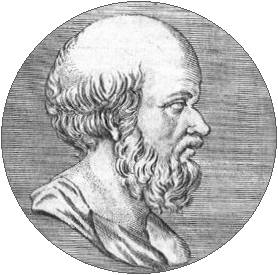
\includegraphics[width=0.3\textwidth]{figs/eratostenes.png}
        \caption{Eratóstenes de Cirene}
        \label{p:crivo}
    \end{figure}
	
	Um \textit{crivo} é uma forma de saber quem são os números primos até um determinado limite $n$. O Crivo de Eratóstenes funciona de forma bem simples:
	\begin{enumerate}
		\item Escrevemos em uma tabela todos os números de 0 até $n$.
		\item Riscamos o 0 e o 1. Começamos do 2.
		
		\item Se um número não estiver riscado, riscamos todos os múltiplos deste, menos o próprio.
		
		\item Andamos para o próximo número e repetimos a etapa anterior.		
	\end{enumerate}
	Uma maneira interessante de fazer isso é criando uma lista de tamanho $n + 1$, ou seja, cujos índices vão de 0 até $n$. \par

	\proposal Implemente o crivo de Eratóstenes e, em seguida, elabore versões melhoradas do algoritmo, até onde conseguir.

    \end{problem}

    \section*{Dicionários}

   